% Modified for use with JCC - Madhusudan Singh Copyright (C) (2012). All rights reserved.
\documentclass[12pt]{article}

\setlength{\oddsidemargin}{0in}  %left margin position, reference is one inch
\setlength{\textwidth}{6.5in}    %width of text=8.5-1in-1in for margin
\setlength{\topmargin}{-0.5in}    %reference is at 1.5in, -.5in gives a start of about 1in from top
\setlength{\textheight}{9in}     %length of text=11in-1in-1in (top and bot. marg.) 
\newenvironment{wileykeywords}{\textsf{Keywords:}\hspace{\stretch{1}}}{\hspace{\stretch{1}}\rule{1ex}{1ex}}

\usepackage{amsmath,amssymb}
\usepackage{graphicx}% Include figure files
%\usepackage{caption}
\usepackage{color}% Include colors for document elements
\usepackage{dcolumn}% Align table columns on decimal point
%\usepackage{bm}% bold math
\usepackage[numbers,super,comma,sort&compress]{natbib}
%\usepackage[nolists, nomarkers, figuresfirst]{endfloat}

\definecolor{background-color}{gray}{0.98}

\title{istar: Software-as-a-Service Platform for Large-Scale Protein-Ligand Docking}
\author{Hongjian Li, Kwong-Sak Leung and Man-Hon Wong\thanks{The authors are with Department of Computer Science and Engineering, Chinese University of Hong Kong}}

\begin{document}

\maketitle


\begin{abstract}
We were motivated by the desire to automate large-scale protein-ligand docking using our idock and thus have developed istar, a general SaaS (Software as a Service) platform. Without tedious software installation, users, especially computational chemists, can submit jobs on the fly either by browsing our web site or by programming against our RESTful API. Our HTML5- and CSS3-powered web site supports 1) selecting ligands with desired molecular properties and previewing the number of ligands to dock, 2) monitoring job progress in real time, and 3) outputing supplier information, three very useful features commonly lacked on other online docking platforms like DOCK Blaster or iScreen. We have collected 12,171,187 yuck-free ligands from the clearn subset of ZINC with conditional permission from its developer. We have developed idock 1.6 for istar, further improving docking speed and accuracy, inventing new functionalities, and fixing bugs. To better evaluate and compare idock 1.6 with the state-of-the-art AutoDock Vina 1.1.2, we have carried out a redocking benchmark on the 2,455 protein-ligand complexes of the refined set of PDBbind v2011 and 343 protein-ligand complexes of CSAR NRC HiQ Set 24Sept2010, and a virtual screening benchmark on 12 diverse receptors and 3000 ligands of different molecular weight. The results have shown that under various circumstances idock displayed comparable success rates but outperformed AutoDock Vina in terms of docking speed by at least 8.69 times and at most 37.51 times, rendering idock particularly suitable for large-scale protein-ligand docking. We have developed an istar-customized daemon from idock 1.6, implementing two-phase docking and exploiting fine-grained slice-level parallelism in order to further shorten job execution time, as well as using gzip to compresses result files in order to save server storage and network bandwidth. We have tested the istar web site with Chrome 19+, Firefox 12+, IE 9+, Safari 5+ and Opera 12+. We have also prepared two graphical tutorials for newbies to get started easily. We plan to utilize GPU acceleration in a future release of idock and deploy GPU clusters for further speed up, aiming to make istar a really pragmatic large-scale online docking platform for the computational chemistry community and pharmaceutical companies.
\end{abstract}

\begin{wileykeywords}
docking, virtual screening, web.
%A list of five key words or phrases which best characterize the paper are required for indexing.
\end{wileykeywords}

\clearpage

%*****************Graphical Table of Contents******************** THIS IS MANDATORY *******************


\begin{figure}[h]
\centering
\colorbox{background-color}{
\fbox{
\begin{minipage}{1.0\textwidth}
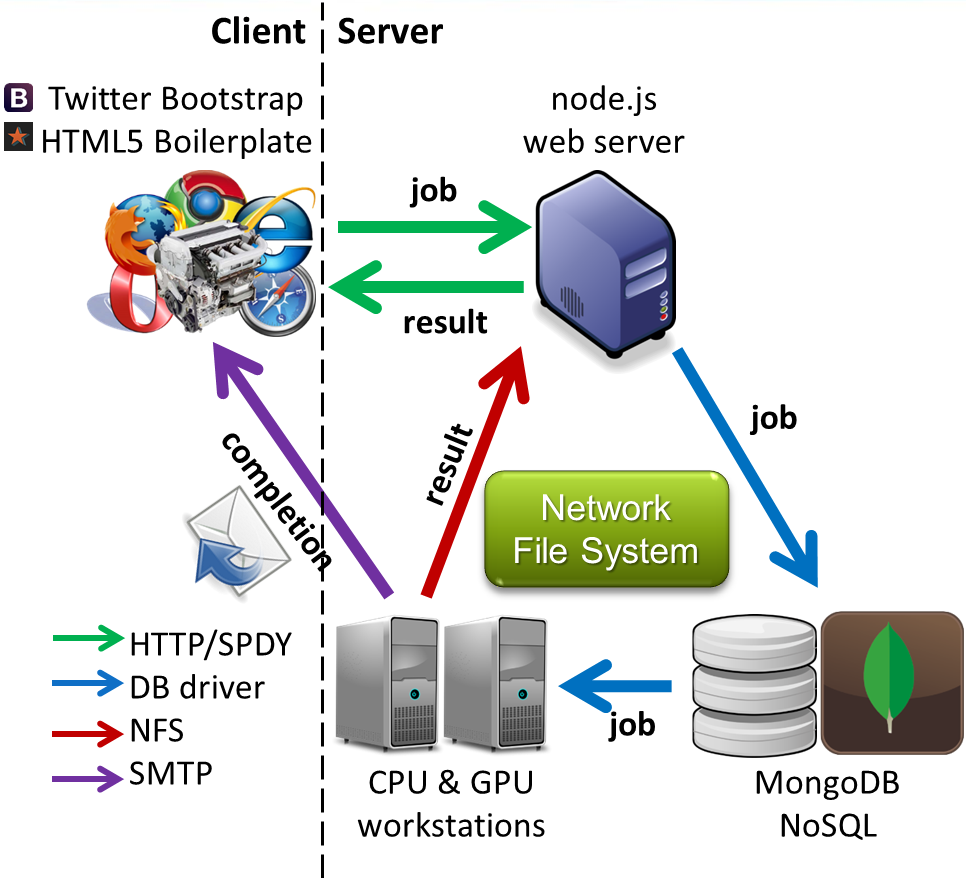
\includegraphics[width=55mm,height=50mm]{GTOC.png} % Pick only one of the two styles by uncommenting the corresponding \includegraphics
%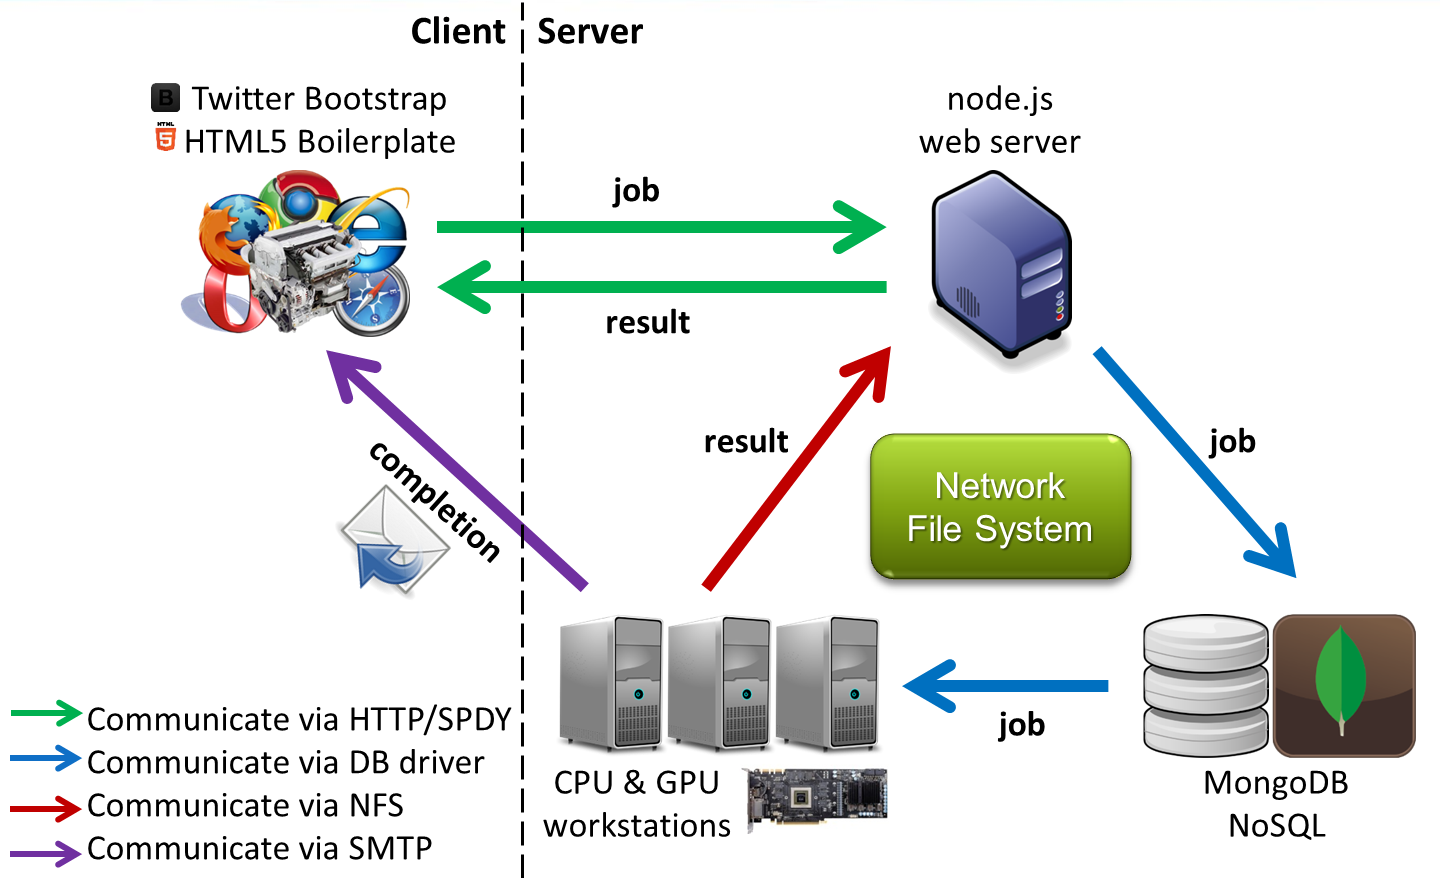
\includegraphics[width=110mm,height=20mm]{Architecture.png}
\\
(75 words.) Images for the graphical Table of Contents should capture the essence of a paper, displaying a figure, plot, or scheme that is central to the theme of the manuscript. The text of the graphical Table of Contents is meant for the non-specialist and should ideally contain no obscure jargon or mathematical symbols / equations, but should attempt to convey the gist of the paper in everyday terms, while remaining consistent with accepted standards of scientific literature.
\end{minipage}
}}
\end{figure}

% makes references listed with 1., 2., etc.  
  \makeatletter
  \renewcommand\@biblabel[1]{#1.}
  \makeatother

\bibliographystyle{apsrev}

\renewcommand{\baselinestretch}{1.5}
\normalsize


\clearpage


\section*{\sffamily \Large SUMMARY}

We have developed istar, a general SaaS (Software as a Service) platform for online large-scale protein-ligand docking. Without tedious software installation, users can submit jobs on the fly either by browsing our web site or by programming against our RESTful API. Our HTML5- and CSS3-powered web site supports 1) selecting ligands with desired molecular properties and previewing the number of ligands to dock, 2) monitoring job progress in real time, and 3) outputing supplier information, three very useful features commonly lacked on other online docking platforms like DOCK Blaster \citep{557} or iScreen \citep{899}. We have collected 12,171,187 yuck-free ligands from the clearn subset of ZINC \citep{1178} with conditional permission from its developer. We have developed idock 1.6 for istar, further improving docking speed and accuracy, inventing new functionalities, and fixing bugs. We have developed an istar-customized daemon from idock 1.6, implementing two-phase docking and exploiting fine-grained slice-level parallelism in order to further shorten job execution time, as well as using gzip to compresses result files in order to save server storage and network bandwidth. We have tested the istar web site with Chrome 19+, Firefox 12+, IE 9+, Safari 5+ and Opera 12+. We have also prepared two graphical tutorials for newbies to get started easily.

\section*{\sffamily \Large INTRODUCTION} % Not needed for rapid communications

Protein-ligand docking predicts the preferred conformation and binding affinity of a small ligand when it is non-covalently bound to a specific binding site of a macro protein. Inspired by AutoDock Vina \citep{595}, we have developed idock 1.0 \citep{1153}, a multithreaded virtual screening tool for flexible ligand docking. idock inherits from AutoDock Vina the accurate scoring function and the efficient optimization algorithm, and meanwhile introduces a list of fruitful innovations, such as receptor and grid map caching for large-scale virtual screening, revised numerical model for much faster approximation, capability of automatic detection and deactivation of inactive torsions, utilization of our novel thread pool to parallelize grid map creation and reuse threads, utilization of modern C++11 features like right-value references to avoid frequent memory reallocation, and accelerated parsers for both receptor and ligand. When benchmarked on docking 10,928 drug-like ligands against HIV-1 reverse transcriptase, idock 1.0 achieved a speedup of 3.3 in terms of CPU time and a speedup of 7.5 in terms of elapsed time on average compared to AutoDock Vina.

Despite the amazing speedup, idock 1.0 required about 10 hours to dock 10,928 drug-like ligands, not to mention massive docking of millions of ligands. Faster implementations are highly desired. Therefore we have developed idock 1.6, further improving docking speed and accuracy, inventing new functionalities, and fixing bugs. Refer to the idock web site for a full list of enhancements and bugfixes.

Having released idock, we kept receiving docking requirements from our colleagues and collaborators. They are mostly biochemists and pharmacists, outsourcing the docking research to us after discovering potential biological targets for certain diseases of therapeutic interest. All of a sudden, we had to grab the protein structure, do format conversion, define search space, set up docking parameters, and keep running idock in batch for months. Tedious enough, all the above work was done manually, resulting in very low research productivity. In order to boost efficiency and automate large-scale protein-ligand docking using our idock, we therefore developed istar, a general SaaS platform.

\section*{\sffamily \Large METHODOLOGY}

Figure \ref{istar:architecture} shows the architecture of istar. There are five major components: a web site, a web server, a database management system, several workstations, and a network file system. Under typical circumstance, a user browses our web site and submits a job. The web server first validates user input and then saves it into database. Several workstations run daemons in the background, fetching jobs from the database and carrying out experiments. Upon completion, they send a notification email to the user and write the result to the network file system, which is served and cached as static content. The user again browses our web site to download result.

\begin{figure}
\centerline{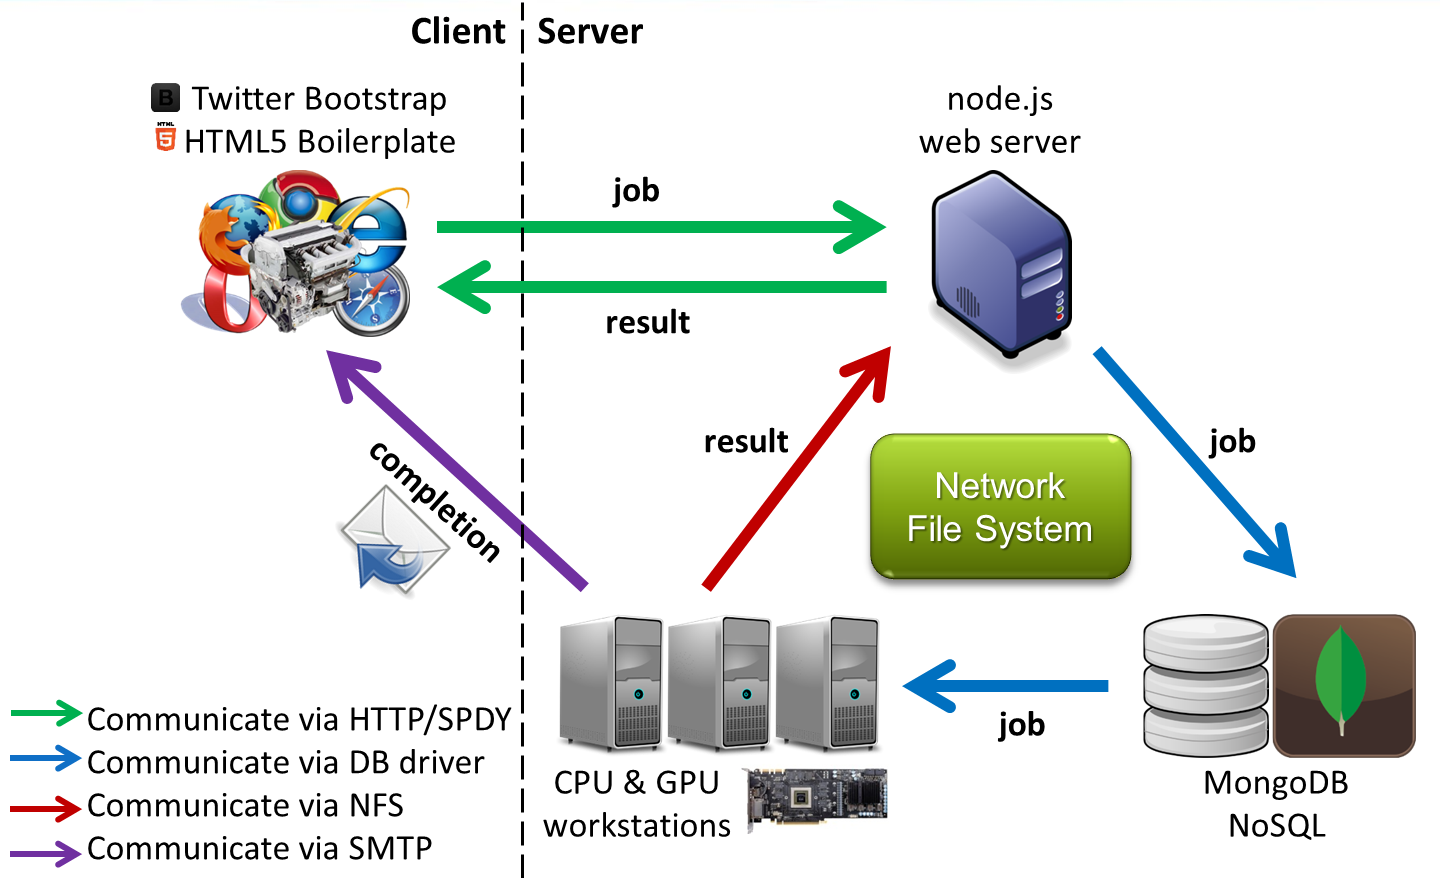
\includegraphics[width=\linewidth]{Architecture.png}}
\caption{istar architecture.}\label{istar:architecture}
\end{figure}

On the client side, we seamlessly combined both the Twitter Bootstrap and the HTML5 Boilerplate into a HTML5- and CSS3-powered web site, which was successfully checked as HTML5 by the W3C Markup Validator v1.3. We adopted the jQuery library to simplify HTML document traversing, event handling, animating, and Ajax interactions, and the jQuery UI library to provide themeable widgets. We tested our web site with Chrome 19+, Firefox 12+, Internet Explorer 9+, Safari 5+ and Opera 12+.

On the server side, we built the web server using the well-known asynchronous event-driven node.js on top of the express server, forking multiple worker processes to accept simultaneous HTTP/SPDY connections. We utilized the spdy node module to support SPDY protocol v3, the prototype of next generation HTTP 2.0, achieving reduced latency through compression, multiplexing, and prioritization. We employed the forever node module to restart worker processes automatically in case of unhandled exceptions, ensuring high availability. We made heavy use of regular expressions and developed a customized validator to validate and sanitize user input, ensuring data validity.

On the database side, we chose MongoDB, a scalable, high-performance, open source NoSQL database. MongoDB features document store in JSON style, making it particularly suitable for applications requiring flexible document attributes like our istar.

On the workstation side, we deployed a Linux workstation and four Mac workstations. The Linux workstation is equipped with Intel Xeon W3520 @ 2.66 GHz, 8GB DDR3 SDRAM and GeForce GTX 285 (1024 MB), and running Fedora 17 x64. The four Mac workstations are equipped with Intel Core i5-2400 @ 3.10GHz and 4GB DDR3 SDRAM, and running Mac OS X Lion 10.7.4.

On the network file system side, we mounted a 2TB hard disk for shared use. All the five workstations can simultaneously access to the hard disk and perform file reading and writing. In principle, we will persist existing jobs and results until storage shortage.

\section*{\sffamily \Large RESULTS}

%((Place Results here. Not needed for review articles.))

\section*{\sffamily \Large First-order heading}
 
%((Equations should be inserted using standard LaTeX equation and eqnarray environments, not as graphics, and should be set in the main text))
%Equation											(1)
%((References should be superscripted and appear after punctuation.1,2 Please define all acronyms at their first usage except IR, UV, NMR, and DNA or similar commonly understood terms.)) 


\subsection*{\sffamily \large Second-order heading}

\subsubsection*{\sffamily \normalsize Third-order heading}

{\sffamily \small Fourth-order heading}\\

\section*{\sffamily \Large DISCUSSION}

DOCK Blaster \citep{557}, an expert system, was created to investigate the feasibility of full automation of large-scale protein-ligand docking. Here we highlight the advantages of istar over DOCK Blaster. First and foremost, istar is free and open source under Apache License 2.0. Everyone is welcome to download a copy and deploy istar to his/her own servers. istar is designed as a general SaaS platform. It can host not only idock but also igrep and any other program. istar utilizes HTML5, CSS3, node.js, SPDY, NoSQL, GPU acceleration and so on, representing a state-of-the-art platform. istar supports filtering and previewing ligands to dock, as well as monitoring job progress in real time, two very useful features only available at istar. istar implements 2-phase docking and exploits fine-grained slice-level parallelism in phase 1.

Due to limited budget, we could not offer hardware resource as much as DOCK Blaster did (i.e. 700 CPU cores plus 20TB RAID-6 storage), so we tried every endeavor on software optimization. Alternatively, one can freely deploy a copy of istar. In the future we plan to port idock to GPU in order to further boost performance.

%\section*{\sffamily \Large CONCLUSIONS}

%((Place Conclusions here.))

\subsection{Availability}
Both idock and istar are free and open source under Apache License 2.0. For idock, its C++ source code, precompiled executables for 32-bit and 64-bit Linux, Windows, Mac OS X, FreeBSD and Solaris, 13 docking examples, and a doxygen file for generating API documentations are available at https://github.com/HongjianLi/idock. For istar, its C++ and JavaScript source code is available at https://github.com/HongjianLi/istar. A live demo is running at http://istar.cse.cuhk.edu.hk.

\subsection*{\sffamily \large ACKNOWLEDGMENTS}

We thank Professor John J. Irwin, the developer and maintainer of ZINC, for granting us permission to use ZINC with three conditions:
\begin{enumerate}
\item We shall provide links to http://zinc.docking.org/substance/zincid for top hits so that users can seek for the most current purchasing information at ZINC's official web site.
\item We shall limit the number of top hits for download to 1000 ligands from a single job.
\item We shall update our ligands when ZINC data is updated so that users can benefit from the most current ligand data.
\end{enumerate}

%((Additional Supporting Information may be found in the online version of this article.))

\clearpage

%%%%%%%%%%%%%%%%%%%%%%%%%%%%%%%%%%%%%%%%%%%%%%%%%%%%%%%%%%%%%%%%%%%%%%%%%%%%%%%%%
% BIBLIOGRAPHY

\bibliography{bibtexrefs}   % Produces the bibliography via BibTeX.


%%%%%%%%%%%%%%%%%%%%%%%%%%%%%%%%%%%%%%%%%%%%%%%%%%%%%%%%%%%%%%%%%%%%%%%%%%%%%%%%%

\clearpage
%%%%%%%%%%%%%%%%%%%%%%%%%%%%%%%%%%%%%%%%%%%%%%%%%%%%%%%%%%%%%%%%%%%%%%%%%%%%%%%%%
% FIGURE CAPTIONS

%%%%% FIGURE ---- cc.eps
\begin{figure}
\caption{\label{cc} Place Figure 1 caption here. In the case of reproduced figures in review articles, you must obtain the publisher's permission and state a suitable notice here along with a citation.}
\end{figure}

\begin{figure}
\caption{\label{fig2} Place Figure 2 caption here. Figures should be uploaded as individual files, preferably .tif or .eps files, at high enough resolution (600 to 1200 dpi) to ensure clarity. Please see the author’s guide for more details and specifications. For high quality illustrations, we highly recommend the use of the TikZ package.}
\end{figure}


%%%%%%%%%%%%%%%%%%%%%%%%%%%%



%%%%%%%%%%%%%%%%%%%%%%%%%%%%%%%%%%%%%%%%%%%%%%%%%%%%%%%%%%%%%%%%%%%%%%%%%%%%%%%%%
% FIGURE FILES

\clearpage

%\vspace*{0.1in}   %%% FIGURE 1
\begin{center}
%\includegraphics[width=0.2\columnwidth,keepaspectratio=true]{cc.eps}
\end{center}
\vspace{0.25in}
\hspace*{3in}
{\Large
\begin{minipage}[t]{3in}
\baselineskip = .5\baselineskip
Figure 1 \\
Author A, Author B, Author C, Author D \\
J.\ Comput.\ Chem.
\end{minipage}
}

\clearpage

\begin{table}
\begin{tabular}{|c|c|c|c|}\hline
\textbf{Quantity} & \textbf{Calculated} & \textbf{Observed} & \textbf{Error} \\ \hline
  Density & 5.3 & 6.3 & Within limits \\ \hline
  Optical magnification & 8.3 & 90.9 & Utterly unacceptable\! \\ \hline
\end{tabular}
\caption{\label{tbl1} Place table caption here.}
\end{table}

\end{document}

